\documentclass[tikz]{standalone}
% \usetikzlibrary{intersections}
\date{}
\usepackage{amsmath,amsthm,amssymb}
\usepackage{xcolor}
\usepackage{tikz}
\usepackage[siunitx]{circuitikz}
\usepackage{tikz-3dplot}
\usepackage{ifthen}
\tikzset{isometricXYZ/.style={x={(-0.866cm,-0.5cm)}, y={(0.866cm,-0.5cm)}, z={(0cm,1cm)}}}
\usetikzlibrary{arrows,decorations.pathmorphing,positioning,fit,trees,shapes,automata,calc,intersections,decorations.markings,patterns,graphs,quotes,plotmarks}
%\usepackage{algorithm}
%\usepackage{algorithmic}
\newcommand{\R}{\mathbb{R}}
\newcommand{\F}{\mathbb{F}}
\newcommand{\bmat}[1]{\begin{bmatrix}#1\end{bmatrix}}
\newcommand{\xth}[1]{{#1}^{\mathrm{th}}}
\newcommand{\pd}[2]{\frac{\partial #1}{\partial #2} }
\newcommand{\pdd}[2]{\frac{\partial^2 #1}{\partial #2^2}}
\newcommand{\myitemsep}{\setlength\itemsep{-0.25em}}
\newcommand{\bigpar}[1]{\left( #1\right)}
\tikzset{myedge/.style={ thick,->,>=stealth',inner sep=0pt,outer sep=3pt}}
\tikzset{hv path/.style= {to path={-| (\tikztotarget)}}}
\tikzset{vh path/.style= {to path={|- (\tikztotarget)}}}

%%%%%%%%%% Using shift and rotate around:

\newcommand{\spring}[4]{
\path[shift={#1},rotate={#2},fill = white,opacity=1.0] (-0.25,-0.5) rectangle (0.25,0.5); % cover
\draw[thick,shift={#1},rotate={#2}] (0,0.5) -- +(0.25,-0.1) -- +(-0.25,-0.2)-- +(0.25,-0.3)-- +(-0.25,-0.4)-- +(0.25,-0.5)-- +(-0.25,-0.6)-- +(0.25,-0.7)-- +(-0.25,-0.8)-- +(0.25,-0.9) -- +(0,-1.0);
\draw[thick,shift={#1},rotate={#2}] (#3,0) node {#4};
}
\newcommand{\ground}[3]{
\draw[thick,shift={#1},rotate={#2}] (-0.5*#3cm,0) -- (0.5*#3cm,0);
\path[thick,shift={#1},rotate={#2},pattern=north west lines] (-0.5*#3cm,0) rectangle (0.5*#3cm,0.2);
}
\newcommand{\dashpot}[4]{
\path[shift={#1},rotate={#1},fill = white,opacity=1.0] (-0.25,0) rectangle (0.25,0.15);
\path[shift={#1},rotate={#1},draw,thick] (0,0) -- +(0.25,0) -- +(0.25,0.25) +(0.15,0.15) -- +(-0.15,0.15)  +(-0.25,0.25) -- +(-0.25,0) -- +(0,0);
\draw[thick,shift={#1},rotate={#1}] (#3,0) node {#4};
}
\newcommand{\mydashpot}[5]{
\begin{scope}[xshift=#1cm,yshift=#2cm,rotate=#3]
	\path[fill = white,opacity=1.0] (-0.25,0) rectangle (0.25,0.15);
	\path[draw,thick] (0,0) -- +(0.25,0) -- +(0.25,0.25) +(0.15,0.15) -- +(-0.15,0.15)  +(-0.25,0.25) -- +(-0.25,0) -- +(0,0);
	\node at (#4,0) {#5};
	\end{scope}
}
\newcommand{\lapof}[1]{\mathcal L \left\{ #1 \right\}}
\newcommand{\lapinv}[1]{\mathcal L^{-1} \left\{ #1 \right\}}
\newcommand{\evalat}[2]{\left. #1 \right|_{#2}}
\newcommand{\myarr}[3]{(-#2:#1) arc (-#2:#2:#1) node[#3] }
\newcommand{\mc}[1]{\mathcal{#1}}
\newcommand{\mred}[1]{\textcolor{red}{[#1]}}
\newcommand{\myco}[2]{\bigpar{ \frac{#1}{#2} }}
\newcommand{\tc}[2]{{#1}{#2}}
\newcommand{\mcb}[1]{{\color{blue}#1}}
\newcommand{\mcr}[1]{{\color{red}#1}}
\newcommand{\mcg}[1]{{\color{green!70!black}#1}}
\usepackage{hyperref}
\hypersetup{colorlinks=true,
linkcolor=blue,          % color of internal links
        citecolor=green,        % color of links to bibliography
          filecolor=magenta,      % color of file links
           urlcolor=blue           % color of external links
}


\begin{document}
\tikzset{help lines/.style=very thin}
\tikzset{Karl's grid/.style={help lines,color=blue!50}}

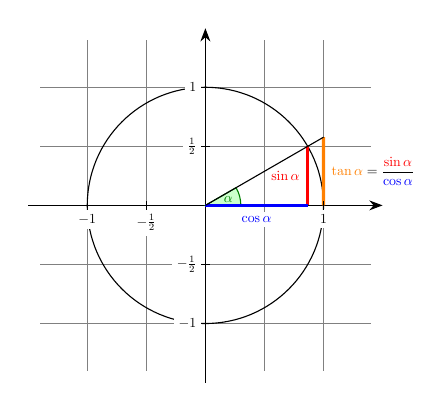
\begin{tikzpicture}[scale=1.5,>=Stealth,every node/.style={scale=0.5}]
%  \clip (-2,-0.2) rectangle (2,0.8);
  \draw[step=0.5cm,gray,very thin] (-1.4,-1.4) grid (1.4,1.4);
  \draw[->] (-1.5,0) -- (1.5,0) coordinate (x axis);
  \draw[->] (0,-1.5) -- (0,1.5) coordinate (y axis);
  \draw (0,0) circle [radius=1cm];
  \filldraw[fill=green!20!white, draw=green!50!black] (0,0) -- (3mm,0mm)
    arc [start angle=0, end angle=30, radius=3mm] -- cycle;
  \draw (15:2mm) node[color=green!50!black] {$\alpha$};
%   \shadedraw[left color=gray, right color=green, draw=green!50!black] (0,0) --
%   (3mm,0mm) arc [start angle=0, end angle=30, radius=3mm] -- cycle;
  \draw[red, very thick] (30:1cm) -- node [left=1pt,fill=white] {$\sin \alpha$}
        (30:1cm |- x axis);
  \draw[blue, very thick] (30:1cm |- x axis) -- node[below=2pt,fill=white] {$
        \cos \alpha$} (0,0);

  \path [name path=upward line] (1,0) -- (1,1);
  \path [name path=sloped line] (0,0) -- (30:1.5cm);
  \draw [name intersections={of=upward line and sloped line, by=t}][very thick,
          orange] (1,0) -- node [right=1pt, fill=white]{$\displaystyle \tan
          \alpha \color{black}=\frac{{\color{red}\sin \alpha}}{{\color{blue}\cos
          \alpha}}$} (t);

  \draw (0,0) -- (t);

  \foreach \x/\xtext in {-1, -0.5/-\frac{1}{2}, 1}
  \draw (\x cm,1pt) -- (\x cm, -1pt) node[anchor=north, fill=white] {$\xtext$};
  \foreach \y/\ytext in {-1,-0.5/-\frac{1}{2},0.5/\frac{1}{2},1}
  \draw (1pt,\y cm) -- (-1pt,\y cm) node[anchor=east, fill=white] {$\ytext$};
\end{tikzpicture}

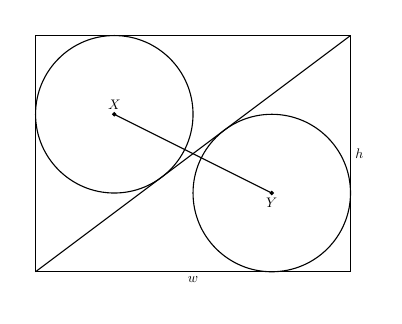
\begin{tikzpicture}[every node/.style={scale=0.5}]
  \clip (-0.1,-0.3) rectangle (4.3,3.1);
  \draw[thin] (0,0) rectangle (4,3);
  \draw (0,0) -- (4,3);
  \draw (1.0, 2.0) circle [radius=1cm];
  \draw (3.0, 1.0) circle [radius=1cm];
  \draw (1.0, 2.0) -- (3.0, 1.0);
  \filldraw (1.0, 2.0) circle [radius=0.2mm];
  \filldraw (3.0, 1.0) circle [radius=0.2mm];
  \draw (1.0,2.0) node[above] {$X$};
  \draw (3.0,1.0) node[below] {$Y$};
  \draw (2.0,0.0) node[below] {$w$};
  \draw (4.0,1.5) node[right] {$h$};
\end{tikzpicture}

\begin{tikzpicture}[scale=1]
\draw (.1,1.6) .. controls (.6,1.6) and (1.5,1) .. (2,1);
\begin{scope}
  \clip (1,0) rectangle (2,2);
  \draw (.1,1) .. controls (.6,1) and (1.5,.4) .. (2,.4);
\end{scope}
\draw[dashed] (1,0) -- (1,2);
\end{tikzpicture}

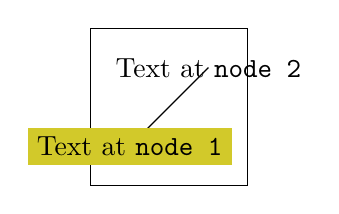
\begin{tikzpicture}
  \draw (0,0) rectangle (2,2);
  \draw (0.5,0.5) node [fill=yellow!80!black]
                       {Text at \verb!node 1!}
     -- (1.5,1.5) node {Text at \verb!node 2!};
\end{tikzpicture}

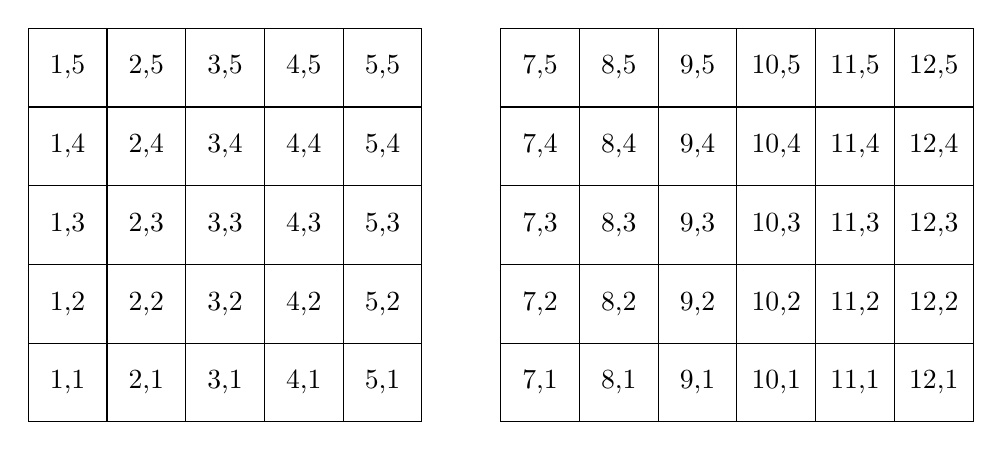
\begin{tikzpicture}[scale=1]
  \foreach \x in {1,2,...,5,7,8,...,12}
    \foreach \y in {1,...,5}
    {
      \draw (\x,\y) +(-0.5,-0.5) rectangle ++(0.5,0.5);
      \draw (\x,\y) node{\x,\y};
    }
\end{tikzpicture}

\end{document}
